\begin{tikzpicture}[
    layer/.style={
        draw=#1!80!black,
        fill=#1!20,
        thick,
        minimum width=4.8cm,
        minimum height=0.72cm,
        inner ysep=4pt,
        align=center,
        rounded corners=3pt,
        font=\footnotesize
    },
    itembox/.style={
        draw=#1!80!black,
        fill=#1!15,
        thick,
        minimum width=5.4cm,
        minimum height=0.72cm,
        inner ysep=4pt,
        align=left,
        rounded corners=3pt,
        font=\footnotesize
    },
    >=stealth
]
    % Software stack layers (left, pitch 1.15cm)
    \node[layer=Salmon]         (app) at (0, 4.60) {\textbf{\faLaptop\hspace{1.5mm}Anwendungen}};
    \node[layer=Goldenrod]      (api) at (0, 3.45) {\textbf{\faPlug\hspace{1.5mm}Systemaufrufe / API}};
    \node[layer=DarkSeaGreen]   (os)  at (0, 2.30) {\textbf{\faCogs\hspace{1.5mm}Betriebssystem}};
    \node[layer=CornflowerBlue] (drv) at (0, 1.15) {\textbf{\faMicrochip\hspace{1.5mm}Gerätetreiber}};
    \node[layer=Gray]           (hw)  at (0, 0.00) {\textbf{\faServer\hspace{1.5mm}Hardware}};

    % Connecting arrows inside stack
    \foreach \from/\to in {app/api, api/os, os/drv, drv/hw} {
        \draw[<->, thick, draw=black!40] (\from) -- (\to);
    }

    % Items to be assigned (right, pitch 1.15cm)
    \node[itembox=DarkSeaGreen]   (iA) at (6.0, 4.60) {\textbf{A}\hspace{2mm}NTFS-Dateisystem};
    \node[itembox=Salmon]         (iB) at (6.0, 3.45) {\textbf{B}\hspace{2mm}Google Chrome (Browser)};
    \node[itembox=Gray]           (iC) at (6.0, 2.30) {\textbf{C}\hspace{2mm}CPU führt Maschinenbefehl aus};
    \node[itembox=CornflowerBlue] (iD) at (6.0, 1.15) {\textbf{D}\hspace{2mm}Grafikkartentreiber};
    \node[itembox=Goldenrod]      (iE) at (6.0, 0.00) {\textbf{E}\hspace{2mm}Aufruf \texttt{open("datei.txt")}};

    % Assignment arrows from items to layers
    \draw[<-, thick, draw=Salmon!80!black]         (app.east) -- (iB.west);
    \draw[<-, thick, draw=Goldenrod!80!black]      (api.east) -- (iE.west);
    \draw[<-, thick, draw=DarkSeaGreen!80!black]   (os.east)  -- (iA.west);
    \draw[<-, thick, draw=CornflowerBlue!80!black] (drv.east) -- (iD.west);
    \draw[<-, thick, draw=Gray!80!black]           (hw.east)  -- (iC.west);

    % Column headers
    \node[above=4pt, font=\scriptsize\bfseries, text=black!70] at (0, 5.0) {Schichten};
    \node[above=4pt, font=\scriptsize\bfseries, text=black!70] at (6.0, 5.0) {Zugeordnete Elemente};
\end{tikzpicture}
